Im Folgenden wird  anhand eines Beispiels illustriert,  wie der Arbeitsprozess
mit unserer Software funktioniert. Dabei werden wir sowohl einen PI-Regler als
auch einen PID-Regler durchrechnen und den Prozess grafisch illustrieren.

Als  Ausgangspunkt  des  Prozesses   dient  die  Schrittantwort  der  Strecke,
aus  welcher  die  Verts\"arkung  $K_s$ der  Strecke,  die  Verz\"ogerungszeit
$T_u$  und die  Anstiegszeit $T_g$  abgelesen werden. Diese  Werte dienen  als
Eingabeparameter unseres Tools.

Wir werden in diesem Bericht folgende Strecke als Beispiel nehmen:
\begin{figure}[h! width=\pagewidth]
    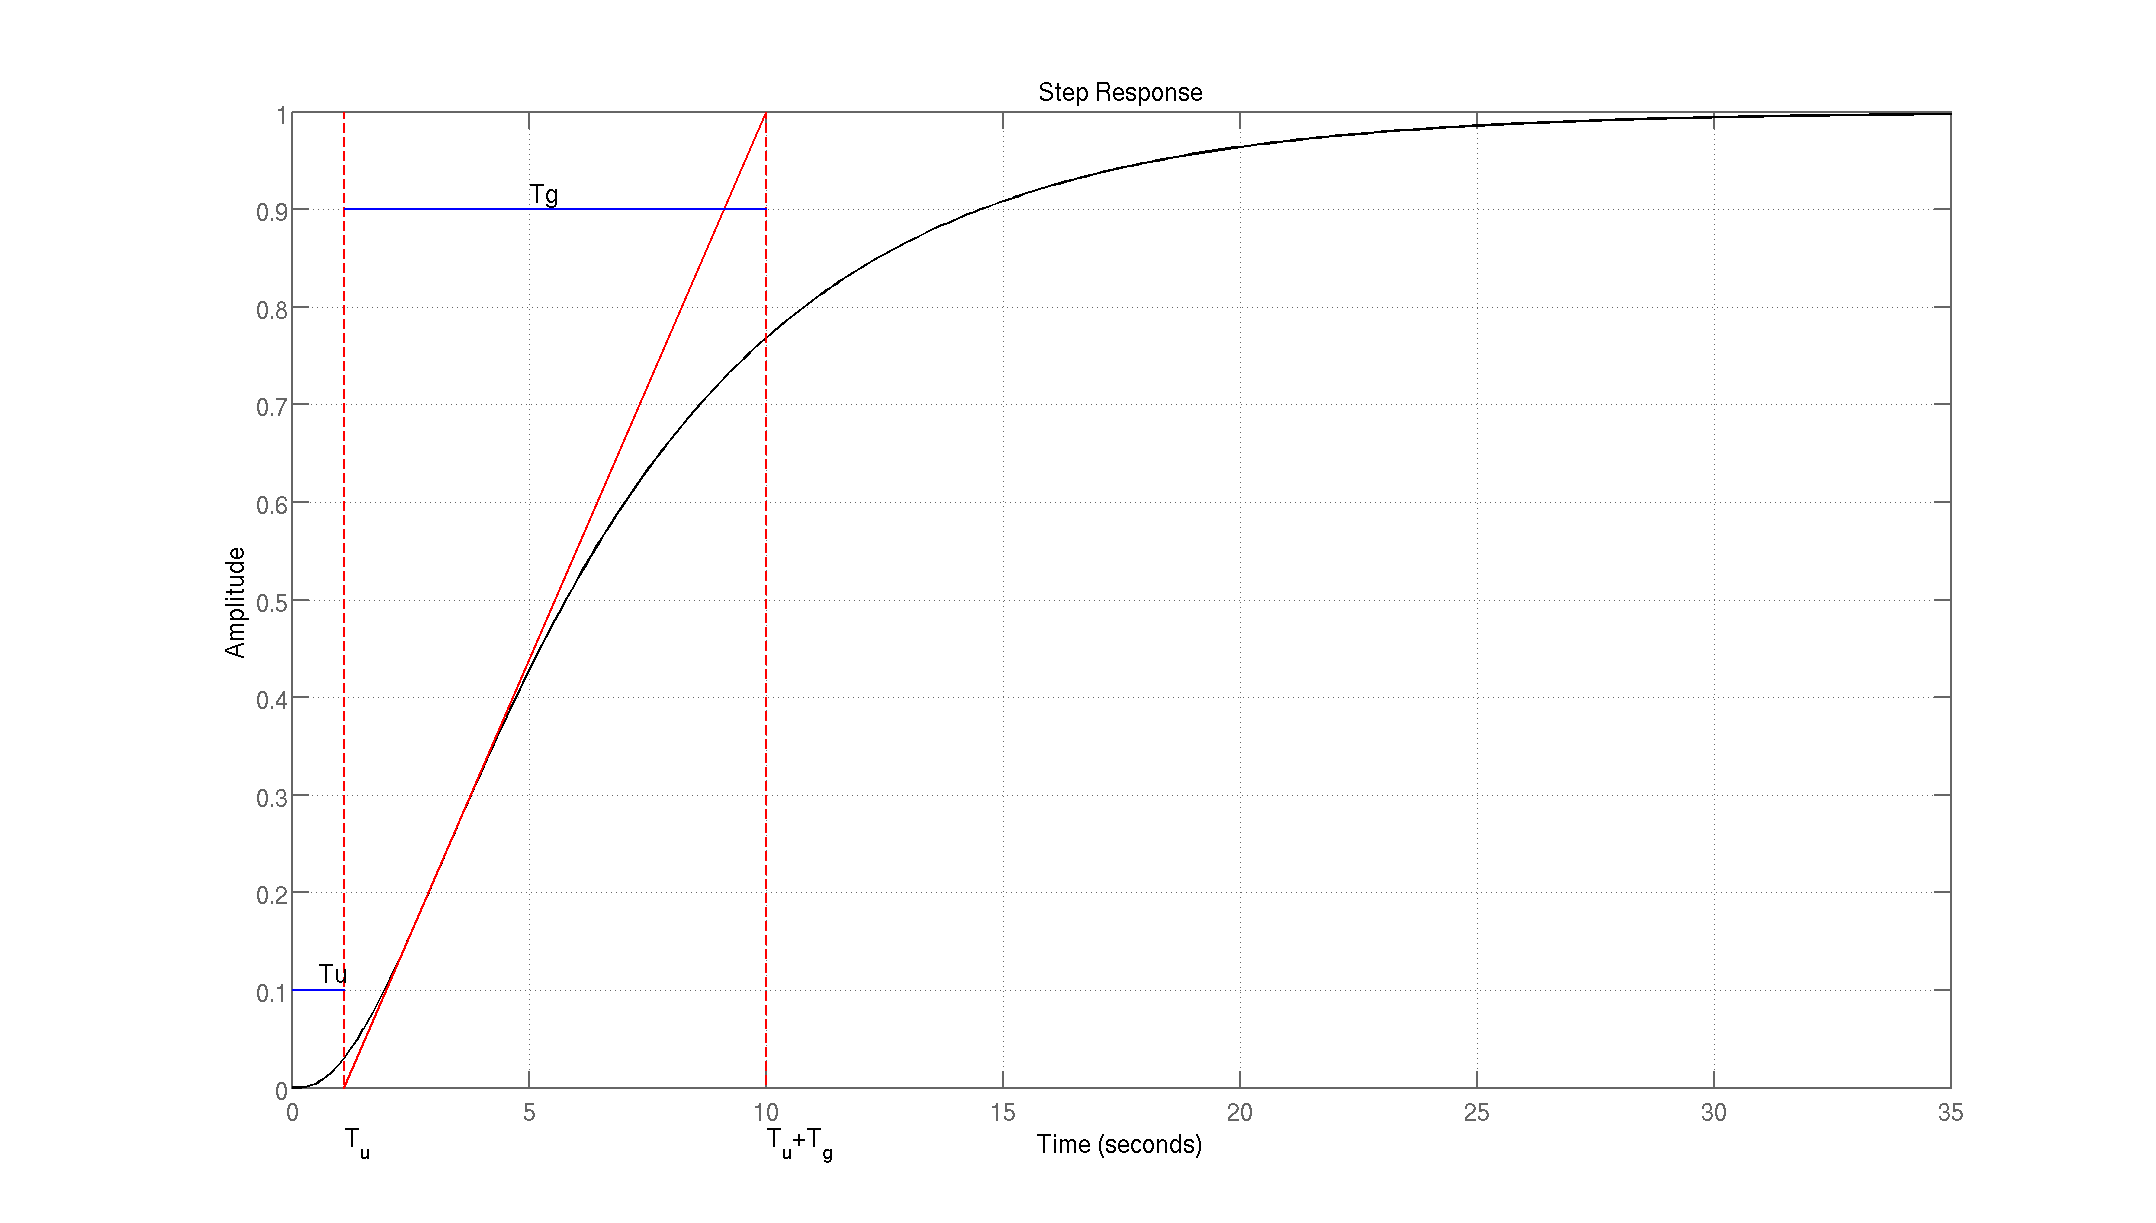
\includegraphics[width=.9\textwidth]{images/streckeSchrittantwort.png}
    \caption{%
    Schrittantwort der  Beispielstrecke (schwarz), Wendetangende  (rot), $T_u$
    und $T_g$ (blau)%
    }
    \label{fig:plant_step}
\end{figure}

Der  geschlossene   Regelkreis  soll  schlussendlich  maximal   etwa  $16.3\%$
\"uberschwingen.

Wir erhalten:
\begin{itemize}
    \item
        $K_s = \SI{2}{\second}$
    \item
        $T_u = \SI{1.1}{\second}$
    \item
        $T_g = \SI{8.9}{\second}$
\end{itemize}

Da  die Phasengangmethode  vom {\em{Frequenzgang}}  einer Strecke  ausgeht und
nicht von der Schrittantwort, besteht der n\"achste Schritt nun darin, aus den
obigen Werten  den Frequenzgang  der Strecke  zu bestimmen. Dies  erledigt die
methode \code{p\_sani}, welche uns  die Werte f\"ur die \"Ubertragungsfunktion
der  Strecke   liefert.  \todo{Allenfalls   Verweis  auf   Softwareteil  f\"ur
Erkl\"arungen  zu  sani-Methode.}   In  unserem  Fall  ergibt  dies  folgendes
Polynom:

\begin{gather} \label{eq:transfer:plant}
    \begin{split}
        H_s (s) & = \frac{1}{1 + s \cdot T_1}
                  + \frac{1}{1 + s \cdot T_2}
                  + \frac{1}{1 + s \cdot T_2}                     \\
                & = \frac{1}{1 + s \cdot \SI{0.4134}{\second}}
                  + \frac{1}{1 + s \cdot \SI{1.4894}{\second}}
                  + \frac{1}{1 + s \cdot \SI{5.3655}{\second}}
    \end{split}
\end{gather}

Mit einem  geeigneten Tool  kann man sich  den dazugeh\"origen  Plot erstellen
lassen.

\begin{figure}[h! width=\pagewidth]
    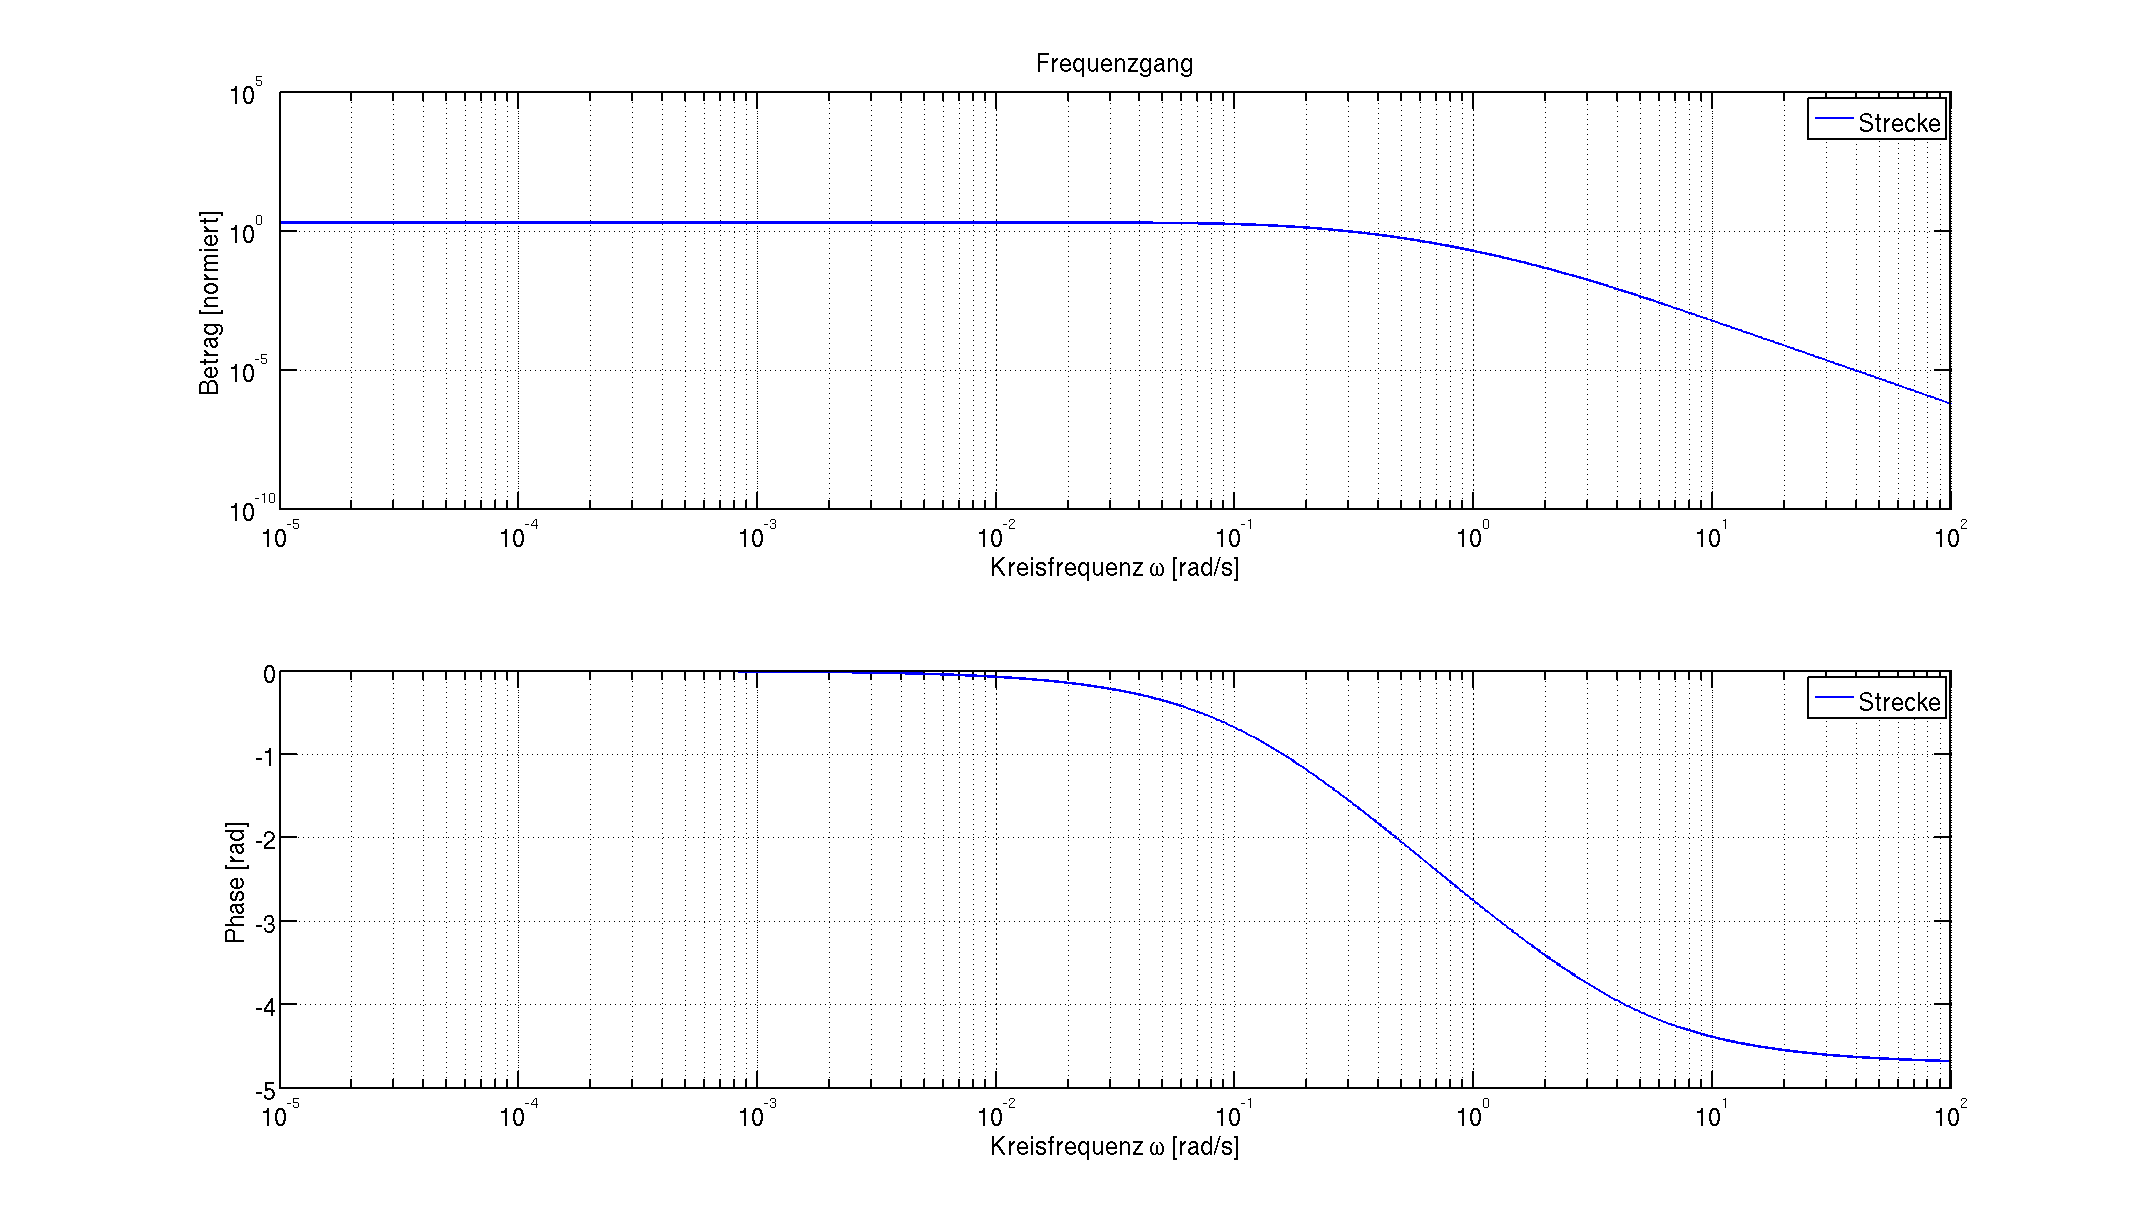
\includegraphics[width=.9\textwidth]{images/streckeFrequenzgang.png}
    \caption{%
        Frequenzgang der Strecke%
    }
    \label{fig:plant_freq}
\end{figure}

An diesem Punkt divergieren die Verfahren f\"ur den PI- und den PID-Regler. Es
soll zuerst der PI-Regler dimensioniert werden.

\subsubsection*{PI-Regler}

Das schlussendliche Ziel ist die Bestimmung der Parameter $K_{rk}$ und $T_{nk}$
in der Gleichung:

\begin{equation} \label{eq:pi:target}
    H_{rpi} = K_{rk} \cdot \Big[ 1 + \frac{1}{s \cdot T_{nk}} \Big]
\end{equation}

Zuerst wird im Phasengang der Strecke die Frequenz $\omega_{pi}$ bestimmt, f\"ur
welche die Phase der Strecke $-90\degree$ betr\"agt.

\begin{equation} \label{eq:pi:phi_s}
    \varphi_s(\omega_{pi}) = -90 \degree
\end{equation}

\begin{figure}[h! width=\pagewidth]
    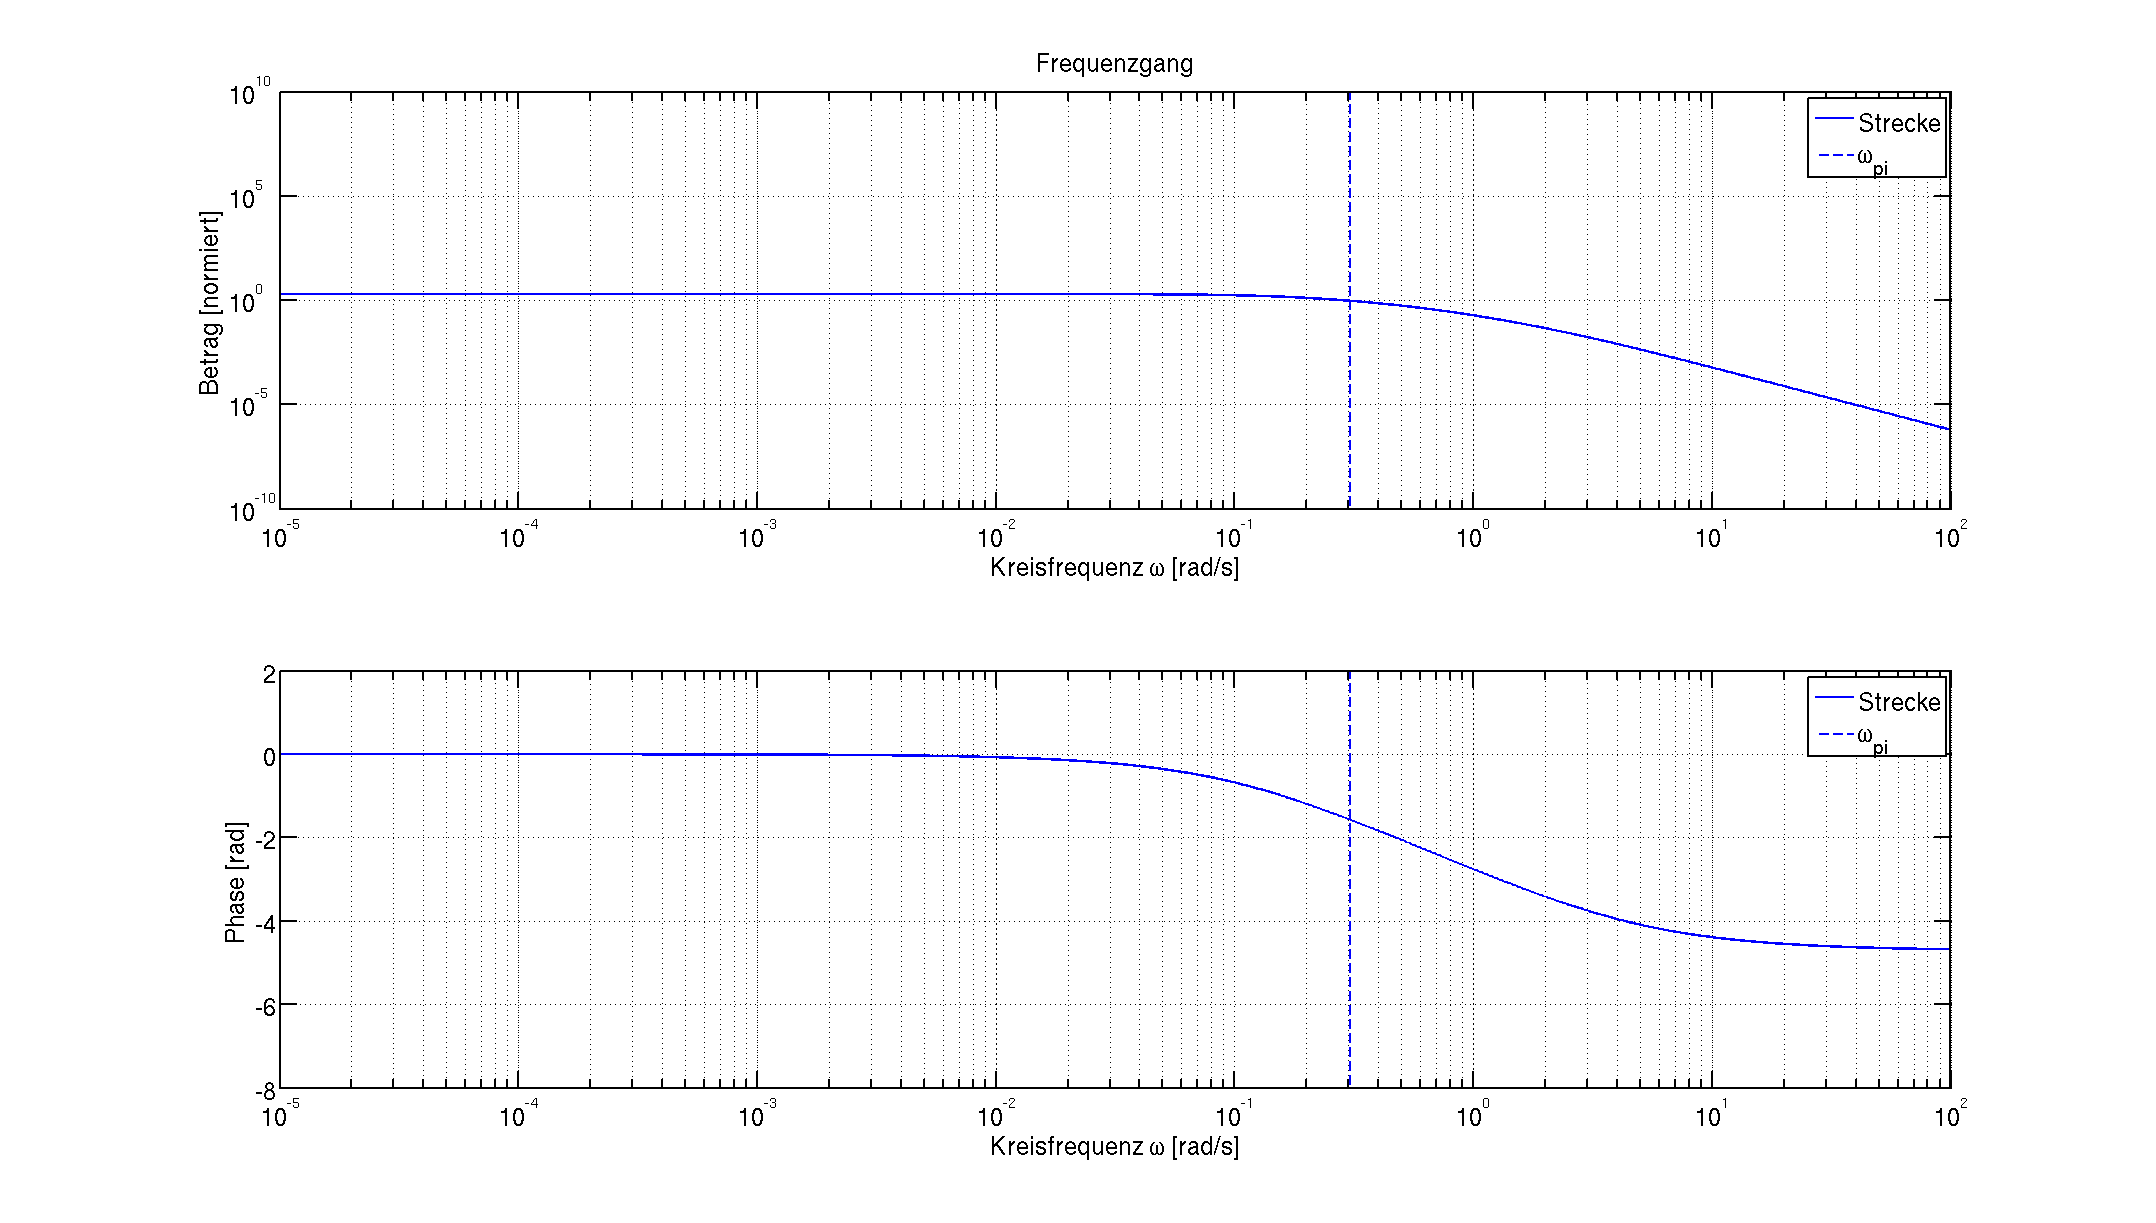
\includegraphics[width=.9\textwidth]{images/piStreckeOmegaPI.png}
    \caption{%
        $\omega_{pi}$ eingetragen (vertikale gestrichelte Linie).
    }
    \label{fig:pi:omega_pi}
\end{figure}

Wie man aus Abbildung \ref{fig:pi:phi_s} ablesen kann, liegt dieser Wert f\"ur
$\omega_{pi}$ in unserem  Beispiel bei ungef\"ahr $\SI{0.3}{\per\second}$. Die
Kontrollrechnung mittels Matlab ergibt:

\begin{equation} \label{eq:pi:omega_pi}
    \omega_{pi} = \SI{0.3039}{\per\second}
\end{equation}

Damit kann nun $T_{nk}$ direkt bestimmt werden\footnotemark[1]:

\begin{equation} \label{eq:pi:omega_pi}
    T_{nk} = \frac{1}{\omega_{pi}} = \frac{1}{\SI{0.3039}{\per\second}} = \SI{3.2902}{\second}
\end{equation}

\footnotetext[1]{
    Um die  Akkumulation von Ungenauigkeiten  zu minimieren werden  bei diesen
    Berechnungen  die  genauen  Werte  aus  Matlab  verwendet  und  nicht  die
    gerundeten  Zwischenresultate,  was  zu   Abweichungen  zu  den  von  Hand
    berechneten Ergebnissen f\"uhren kann.
}
\todo{Fragen ob dies OK ist.}

Als N\"achstes  soll die Durchtrittsfrequenz $\omega_d$  bestimmt werden. Dazu
wird  der  f\"ur  $T_{nk}$  erhaltene  Wert  in  Gleichung  \ref{eq:pi:target}
eingesetzt. Da $K_{rk}$ noch unbekannt ist, wird vorerst $K_{rk} = 1$ gesetzt.

\begin{gather} \label{eq:pi:target}
    \begin{split}
        H_{rpi} & = K_{rk} \cdot \Big[ 1 + \frac{1}{s \cdot T_{nk}} \Big] \\
                & = 1      \cdot \Big[ 1 + \frac{1}{s \cdot \SI{3.2902}{\second}} \Big]
    \end{split}
\end{gather}

Daraus   kann   nun   der   Frequenzgang   des   {\em{offenen   Regelkreises}}
(\"Ubertragungsfunktion $H_o$,  Amplitudengang $A_o$,  Phasengang $\varphi_o$)
bestimmt werden.

\begin{gather} \label{eq:pi:h_open}
    \begin{split}
        H_o (s) & = H_{rpi} (s) \cdot H_s (s) \\
            & = \bigg(
                    K_{rk} \cdot \Big[ 1 + \frac{1}{s \cdot T_{nk}} \Big]
                \bigg)
                \cdot
                K_s
                \cdot
                \bigg(
                        \frac{1}{1 + s \cdot T_1}
                  \cdot \frac{1}{1 + s \cdot T_2}
                  \cdot \frac{1}{1 + s \cdot T_2}
                \bigg) \\
            & = \bigg(
                    1 \cdot \Big[ 1 + \frac{1}{s \cdot \SI{3.2902}{\second}} \Big]
                \bigg)
                \cdot
                2
                \cdot
                \bigg(
                          \frac{1}{1 + s \cdot \SI{0.4134}{\second}}
                    \cdot \frac{1}{1 + s \cdot \SI{1.4894}{\second}}
                    \cdot \frac{1}{1 + s \cdot \SI{5.3655}{\second}}
                \bigg)
    \end{split}
\end{gather}


Wobei der Amplitudengang den Betragsverlauf und der Phasengang den Verlauf des
Arguments dieser \"Ubertragungsfunktion repr\"asentieren:
\todo{Allenfalls auch wirklich ausrechnen... w\"urde aber ziemlich langwierig.}

\begin{equation}
    \begin{split} \label{eq:pi:a_o_phi_o}
        A_o(j\omega)       & = |H_o(j\omega)| \\
        \varphi_o(j\omega) & = arg(H_o(j\omega))
    \end{split}
\end{equation}

Von besonderem  Interesse ist  hier der Phasengang. Wie  Anfangs spezifiziert,
soll  ein maximals  \"Uberschwingen von  ca. $16.3\%$ angestrebt  werden. Dazu
muss die Durchtrittsfrequenz $\omega_d$ gefunden werden, an welcher der offene
Regelkreis eine Phase von $-128.5\degree$ aufweist. \footnotemark[2]

\footnotetext[2]{%
    Wird ein anderes \"Uberschwingverhalten gew\"unscht, muss hier ein anderer
    Wert f\"ur die Durchtrittsfrequenz  $\omega_d$ bestimmt werden, siehe dazu
    Tabelle \ref{tab:phi_s}.
}

\begin{figure}[h! width=\pagewidth]
    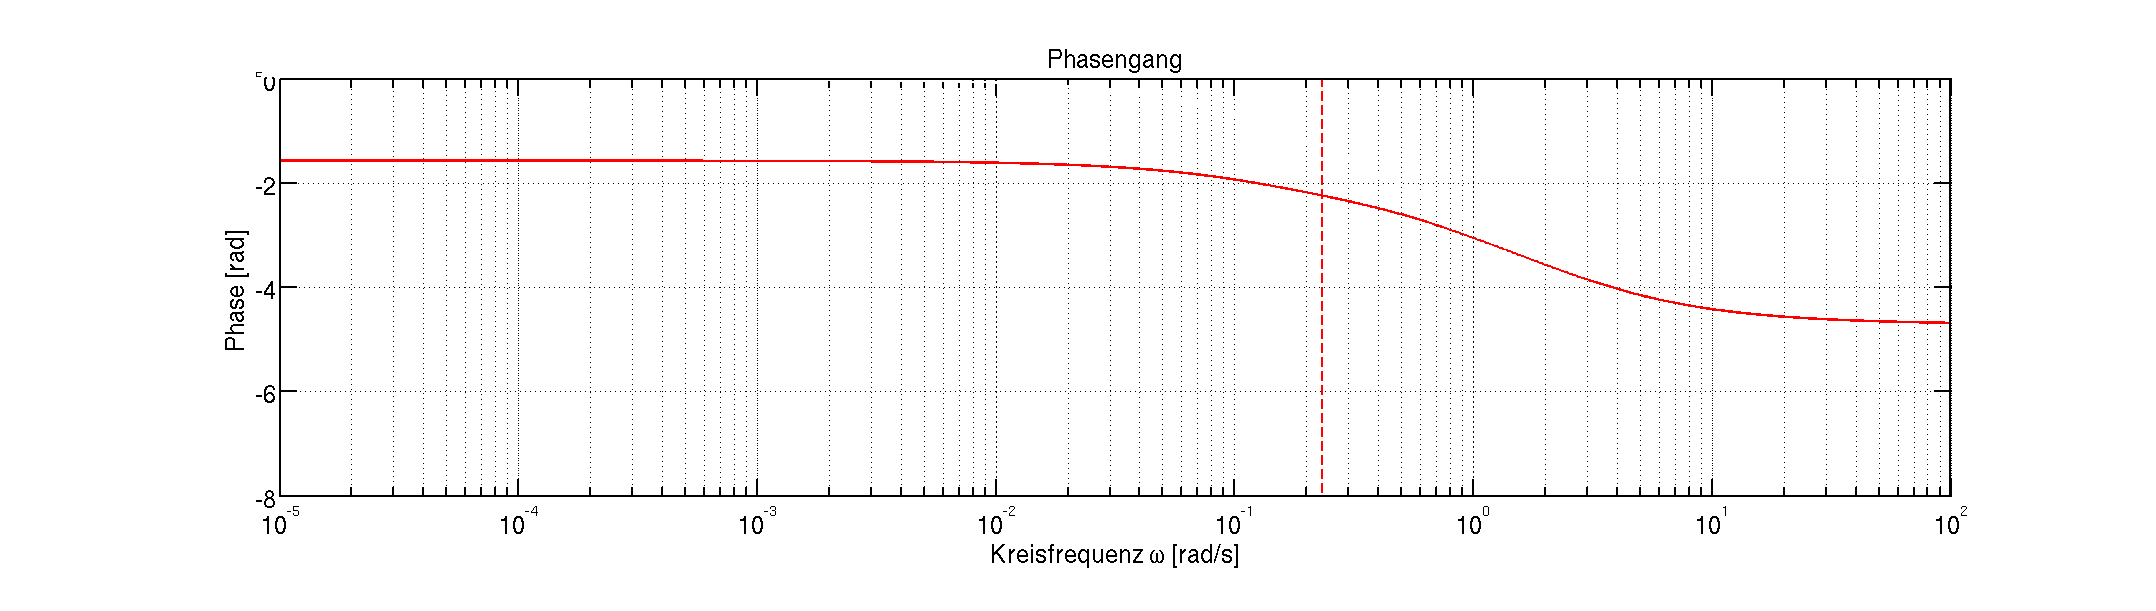
\includegraphics[width=.9\textwidth]{images/piOffenerRegelkreisPhasengang.png}
    \caption{%
        Phasengang   $\varphi_o(j\omega)$   des   offenen   Regelkreises   mit
        eingetragener Durchtrittsfrequenz $\omega_{d}$ (vertikale gestrichelte
        Linie). Wie man verifizieren kann, weist der offene Regelkreis unseres
        Beispiels bei dieser Kreisfrequenz  eine Phase von $-128.5\degree$ auf
        (etwa $\SI{-2.24}{\radian}$).
    }
    \label{fig:pi:omega_d}
\end{figure}

Dies ergibt:
\begin{equation} \label{eq:pi:omega_d}
    \omega_d = \SI{0.2329}{\radian\per\second}
\end{equation}

In  einem  letzten  Schritt  wird  nun  die  Durchtrittsfrequenz  benutzt,  um
die  ben\"otigte Verst\"arkung  $K_{rk}$ des  Reglers zu  bestimmen. Dazu wird
$\omega_d$ in  Gleichung \ref{eq:pi:h_open}  eingesetzt, $|H_o(j\omega)|  = 1$
gesetzt    (Durchtrittsfrequenz: Frequenz,     bei    der     die    Amplitude
$\SI{0}{\decibel} = 1$ ist).

\begin{gather} \label{eq:pi:A_o_set_to_one}
    \begin{split}
        A_o & = | H_o (j\omega_d) | \\
            & = \abs*{
                    \bigg(
                        K_{rk} \cdot \Big[ 1 + \frac{1}{j \cdot \omega_d \cdot T_{nk}} \Big]
                    \bigg)
                    \cdot
                    K_s
                    \cdot
                    \bigg(
                            \frac{1}{1 + j \cdot \omega_d \cdot T_1}
                      \cdot \frac{1}{1 + j \cdot \omega_d \cdot T_2}
                      \cdot \frac{1}{1 + j \cdot \omega_d \cdot T_2}
                      \bigg)} \\
              & = 1
    \end{split}
\end{gather}

Mit den Werten
\begin{equation} \label{eq:pi:values}
    \begin{split}
        K_s      & = 2                    \\
        T_{nk}   & = \SI{3.2902}{\second} \\
        T_1      & = \SI{0.4134}{\second} \\
        T_2      & = \SI{1.4894}{\second} \\
        T_3      & = \SI{5.3655}{\second} \\
        \omega_d & = \SI{0.2329}{\radian\per\second}
    \end{split}
\end{equation}

l\"ost  man Gleichung  \ref{eq:pi:A_o_set_to_one}  nun nach  $K_{rk}$ auf  und
erh\"alt:

\begin{equation} \label{eq:pi:k_rk_result}
    K_{rk} = 0.517577
\end{equation}

Somit ist der PI-Regler vollst\"andig bestimmt und hat folgende Form:

\begin{equation} \label{eq:pi:result}
    H_{rpi} = 0.518 \cdot \Big[ 1 + \frac{1}{s \cdot \SI{3.29}{\second}} \Big]
\end{equation}

Zum Vergleich das Bode-Diagramm mit allen relevanten Kurven und Werten:
\begin{figure}[h! width=\pagewidth]
    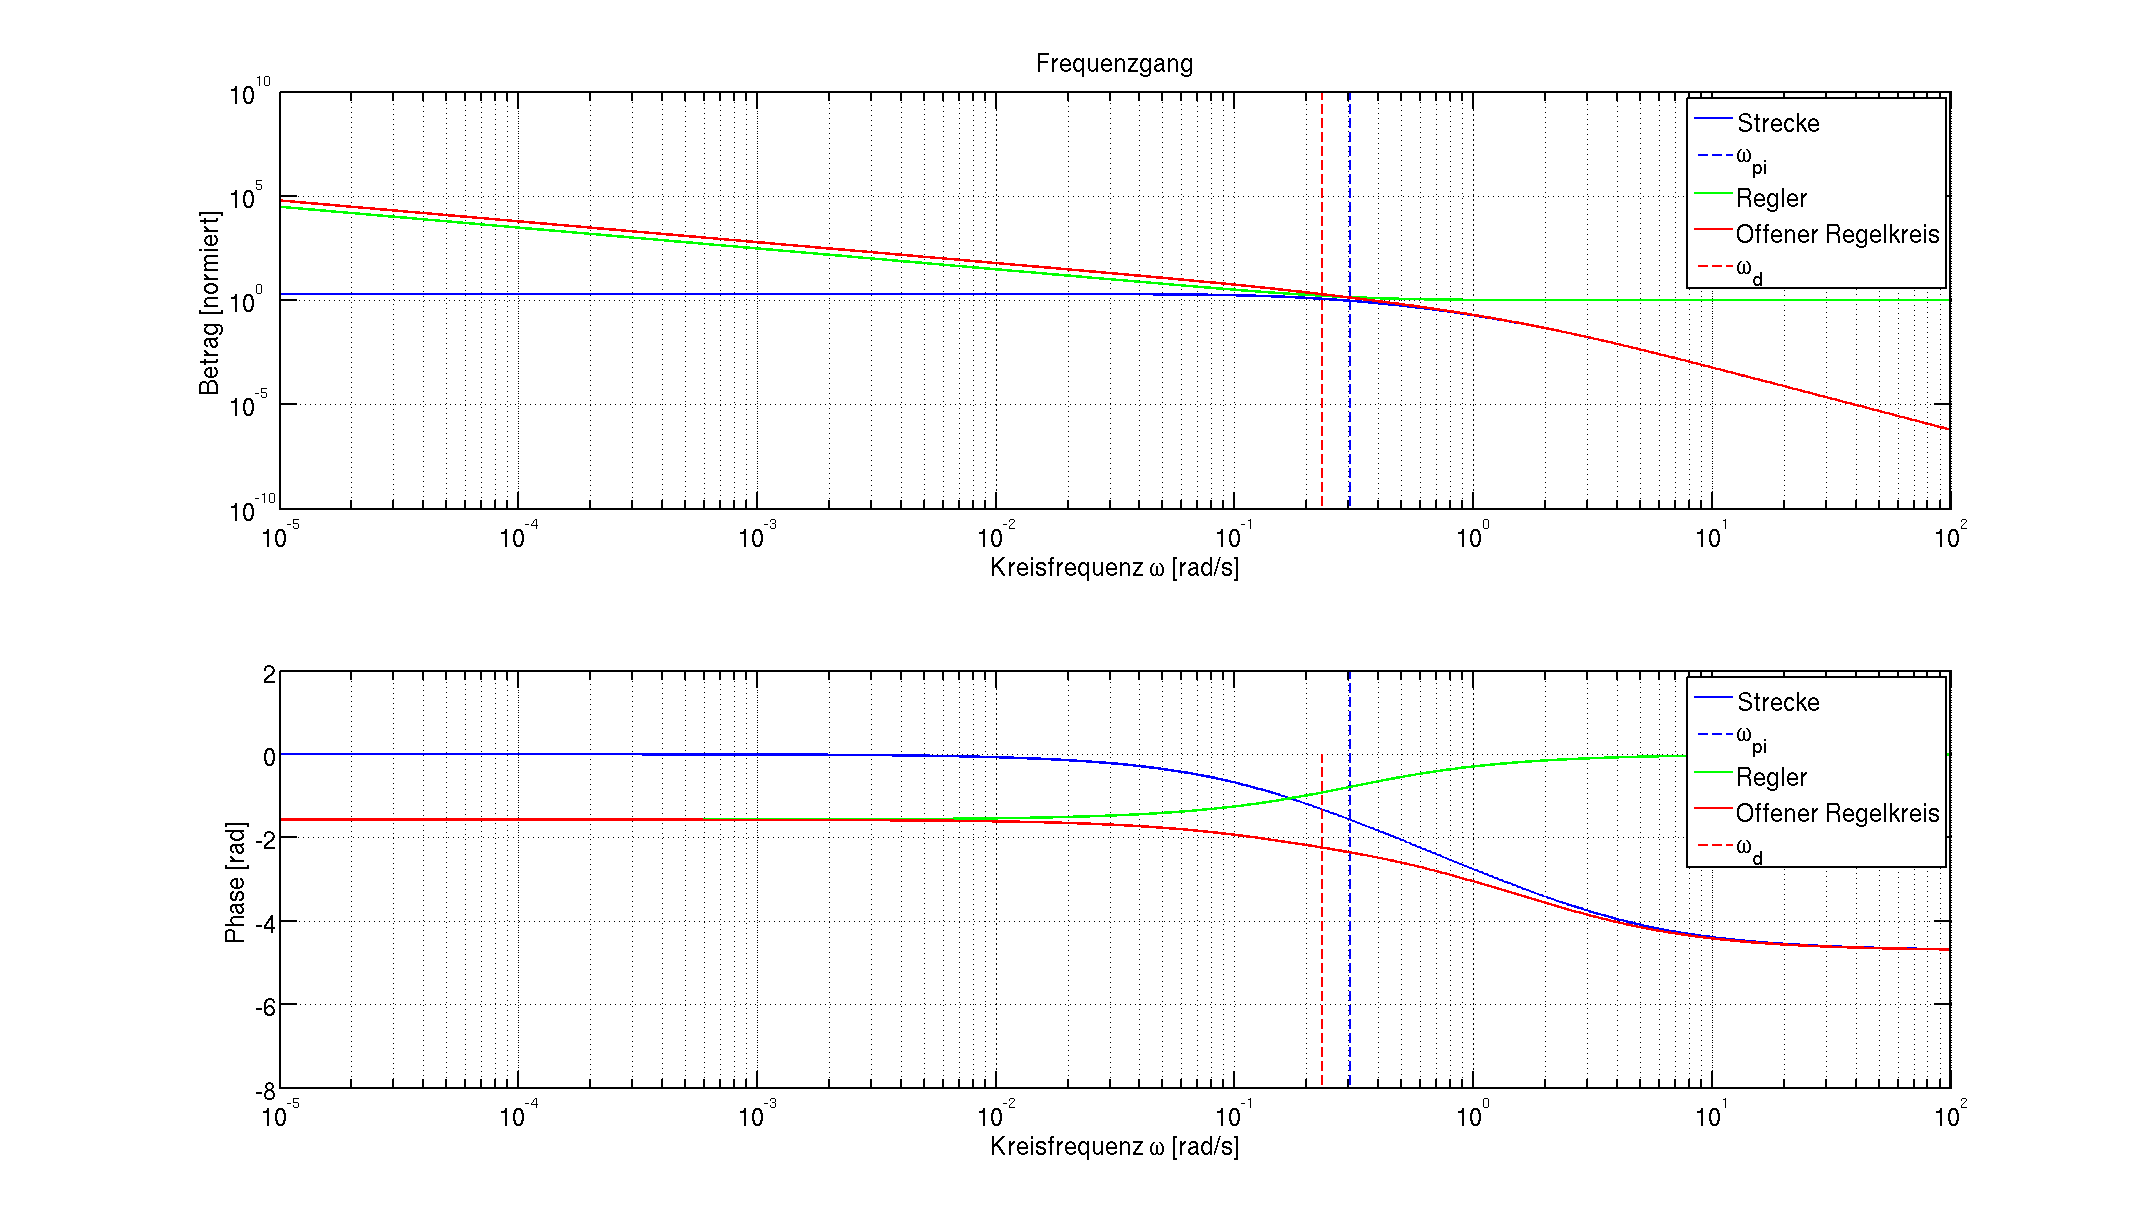
\includegraphics[width=.9\textwidth]{images/piBode.png}
    \caption{%
        Frequenzgang des Reglers (gr\"un), der  Strecke (blau) und des offenen
        Regelkreises (rot).
    }
    \label{fig:pi:all}
\end{figure}
\todo{Fix vertical line $\omega_d$}

\subsubsection*{PID-Regler}
